\documentclass[11pt]{article}
\usepackage[margin=1in]{geometry}
\usepackage{volfit_preamble}
\graphicspath{{figures/}}

\title{\textbf{The Premium You Never Observe}\\[2pt]
\large A lecture on early exercise, optimal stopping, and the subtraction
that removes it from a quote\\[2pt]
\normalsize Vol-Fitter Technical Notes, No.~05}
\author{Vol-Fitter}
\date{\today}

\begin{document}
\maketitle

% Generated numbers.  deam_tables.tex carries the benchmarked kernel timing
% and the worked-example prices (gen_deam.py); deam_stopping_tables.tex the
% figures unique to this edition (gen_deam_stopping.py).  Never retype a
% generated number.
% Auto-generated by gen_deam.py — do not edit.
\newcommand{\deammaxbias}{282}
\newcommand{\deamnumpyms}{12.5}
\newcommand{\deamnumbams}{0.06}
\newcommand{\deamspeedup}{218}
\newcommand{\deamchainn}{300}
\newcommand{\deamsteps}{192}
\newcommand{\deambisect}{24}

% Auto-generated by gen_deam_stopping.py — do not edit.
\newcommand{\deamstmaxbias}{282}
\newcommand{\deamstvegaotmerr}{1.4}
\newcommand{\deamstmapputbdry}{130}
\newcommand{\deamstmapcallbdry}{77}
\newcommand{\deamstmapputeep}{2.7}
\newcommand{\deamstdepthbp}{1.2}
\newcommand{\deamstdepthbpscalar}{0.30}
\newcommand{\deamstrootbp}{0.2}
\newcommand{\deamstdepthshift}{2}
\newcommand{\deamstdepthmax}{2.1}
\newcommand{\deamstalpha}{1.037}
\newcommand{\deamstescrowratio}{3.2}
\newcommand{\deamstcvxbefore}{-1.6}
\newcommand{\deamstcvxaftermant}{-1.7}
\newcommand{\deamstcvxafterexp}{-17}
\newcommand{\deamstcvxmove}{134}
\newcommand{\deamstcvxcore}{0}
\newcommand{\deamstcvxinband}{yes}
\newcommand{\deamstrefagree}{-16}
\newcommand{\deamstrealmedianitm}{519}
\newcommand{\deamstrealmaxbias}{814}
\newcommand{\deamstrealnputs}{120}
\newcommand{\deamstrealnitm}{54}
\newcommand{\deamstliqmant}{2.7}
\newcommand{\deamstliqexp}{-5}
\newcommand{\deamstdepthrealmed}{2}
\newcommand{\deamstdepthrealmax}{8}
\newcommand{\deamstseln}{109}
\newcommand{\deamstselabsmedian}{4.2}
\newcommand{\deamstselmax}{60}
\newcommand{\deamstselputmedian}{10}
\newcommand{\deamstselputmax}{60}
\newcommand{\deamstselcallmedian}{-2.1}
\newcommand{\deamstselcallmax}{1.9}
\newcommand{\deamstgencommit}{5b5b97f}
\newcommand{\deamstgendate}{2026-07-18}
\newcommand{\deamstscalarsteps}{501}


\begin{abstract}
A listed American option quote is the value of an optimal-stopping problem,
not of a terminal expectation --- and every volatility model in this series
prices terminal expectations.  The difference between the two, the
early-exercise premium, is nonnegative, often zero, sometimes hundreds of
basis points of implied volatility, and \emph{never directly observable}:
the market quotes one number, and the premium inside it must be inferred.
This lecture develops the standard desk repair, de-Americanization, as an
exercise in removing an unobservable nuisance with a model in which it
cancels.  We first locate the nuisance: optimal-stopping theory says
exactly when the premium vanishes (never for a call on a name that pays no
dividends --- a theorem of Merton's) and where it concentrates (deep
in-the-money puts under positive rates; calls near dividends), so the whole
strike--maturity plane is mapped before anything is subtracted.  The
subtraction itself is a one-dimensional root find through a
Cox--Ross--Rubinstein tree --- the classical monotone scheme for the
obstacle problem --- and the reason it works is a control-variate identity:
at the root, the model's premium cancels the market's, and most of the
tree's own discretization error cancels between its American and European
legs, leaving the reported quote carrying only the European-leg gap
(\deamstdepthbp\ vol bp at the production batch depth on the worked
example, \deamstdepthbpscalar\ at the scalar depth).  The mathematics is
then held to production discipline: a forward-consistent escrowed
cash-dividend tree, spread-preserving subtraction, loud scalar failures and
silent batch \texttt{NaN} lanes, an \deamspeedup$\times$ compiled kernel
behind an unchanged public dispatch, a content cache that scopes the cost
to genuine data changes, and a wing-only, band-constrained convex repair
for the butterfly arbitrage that per-strike inversion leaves behind ---
including the reverted global repair that taught the locality rule.  On a
synthetic $6\%$-dividend name the naive European inversion is biased by up
to \deamstmaxbias\ vol bp; on a captured SPY chain the same wedge runs to a
median \deamstrealmedianitm\ vol bp --- but only on deep ITM puts the
fitter \emph{discards}; on the quotes production actually fits, the
premium is worth a median $|\cdot|$ of \deamstselabsmedian\ vol bp,
maximum \deamstselmax.  Knowing which of those numbers to quote is, in
miniature, what this note is about.
\end{abstract}

\newpage
\tableofcontents
\newpage

%======================================================================
\section{A quote that lies about volatility}
\label{sec:problem}

Every model in this series prices the same object: the normalized
European call,
\begin{equation}
c(\logm)=\E^{T}\!\big[(e^{X_t}-e^{\logm})^+\big],\qquad
X_t=\log(S_t/\fwd),
\label{eq:normcall}
\end{equation}
a \emph{terminal} expectation under the $t$-forward measure.  A US-listed
single-stock or ETF option is a different asset.  Its holder may exercise at
any moment, so its price is the value of an \emph{optimal-stopping} problem,
and it decomposes as
\begin{equation}
A \;=\; E \;+\; \pi,\qquad \pi\ge0,
\label{eq:decomp}
\end{equation}
where $E$ is the European value the fitter wants and $\pi$ --- the
early-exercise premium --- is the value of the right to stop early.  The
market prints $A$.  It does not print $E$, and it does not print $\pi$:
the decomposition \eqref{eq:decomp} is real but unobservable, quote by
quote.  Feed $A$ into any European inversion and the machinery has no slot
for $\pi$, so it books the whole premium as volatility.  The smile comes
out biased upward --- and, as we will see, biased worst precisely where the
fitter can least afford it.

This note is the story of how the implementation removes $\pi$ without ever
observing it.  The plan of the lecture: first say exactly \emph{where}
$\pi$ lives, using the little optimal-stopping theory that decides when it
is zero (\cref{sec:stopping}); place the removal step inside the quote
pipeline (\cref{sec:pipeline}); build the pricing map --- a
Cox--Ross--Rubinstein tree with a forward-consistent dividend model ---
and establish the monotonicity that makes inversion well posed
(\cref{sec:tree}); expose the inversion as a control variate and account
for every basis point of its error budget
(\cref{sec:cv,sec:budget,sec:example}); count its cost and how production
made that cost vanish (\cref{sec:cost}); repair the one arbitrage the
per-strike construction leaves behind (\cref{sec:convex}); and close with
real-chain evidence, honestly labelled (\cref{sec:real}), what is original
(\cref{sec:original}), and where the guarantees stop (\cref{sec:limits}).

\begin{invariant}
The de-Americanization machinery protects five production invariants:
\begin{enumerate}[leftmargin=1.5em,itemsep=1pt]
\item European chains are untouched --- every step below is a byte-identical
no-op unless the snapshot declares itself American.
\item One premium per strike, subtracted from bid, mid and ask alike: the
quoted \emph{dollar spread} survives de-Americanization.
\item A failed inversion never invents an adjustment: the premium is taken
as zero and the raw band falls through to the European static-bound
filters.
\item The dense at-the-money core is never moved by the convexity repair
(\cref{sec:convex}).
\item Fit settings --- model choice, penalties, weights, optimizer tuning
--- never re-run the trees (the prepared-quote cache, \cref{sec:cost}).
\end{enumerate}
\end{invariant}

\paragraph{Conventions and the notation ledger.}
$S$ is spot; $\fwd$ the forward and $D$ the discount factor to expiry (both
resolved from the chain itself, Note~06); $K$ a strike and
$\logm=\log(K/\fwd)$ its log-moneyness; $r=-\log(D)/t$ and
$q=r-\log(\fwd/S)/t$ the continuously compounded rate and carry yield the
pair $(\fwd,D)$ implies.  $t$ is the \emph{calendar} year fraction to
expiry --- the clock every tree in this note marches on --- and $\tau$ the
event-weighted variance-clock years (Note~00), which appears exactly twice
(\cref{sec:pipeline,sec:cost}).  $\tvar=\sigma^2\tau$ is total implied
variance, $z=\logm/\sqrt{\tvar_{\atm}}$ standardized moneyness.  Dollar
quotes are $P^{\mathrm b}\le P^{\mathrm m}\le P^{\mathrm a}$ (bid, mid,
ask); a \emph{normalized call} is $c=P/(D\fwd)$ plus the parity shift of
\cref{eq:parity}.  One \emph{vol bp} is $10^{-4}$ of absolute volatility.
One differentiation convention throughout: a subscripted $\partial$ is a
partial derivative ($\partial_\sigma\Black$, $\partial_{KK}C$); no primes.

\begin{table}[H]
\centering\footnotesize
\setlength{\tabcolsep}{4pt}
\begin{tabular}{@{}llll@{}}
\toprule
$S,\ \fwd,\ D$ & spot, forward, discount &
$K,\ \logm,\ z$ & strike; $\log(K/\fwd)$; standardized\\[2pt]
$t,\ \tau$ & calendar years; variance-clock years &
$r,\ q$ & rate and carry implied by $(\fwd,D)$\\[2pt]
$A(\sigma),\ E(\sigma)$ & American / European tree price &
$N,\ \Delta t,\ u,\ d,\ p$ & tree depth, step, moves, up-prob.\\[2pt]
$\pi,\ \hat\pi$ & premium $A-E$; its estimate \eqref{eq:eephat} &
$\sigma,\ \sigma^*$ & volatility; the de-Am root \eqref{eq:deam}\\[2pt]
$\Black(\logm,\tvar)$ & normalized Black call &
$c,\ \tvar$ & normalized call; total variance\\[2pt]
$P^{\mathrm b},P^{\mathrm m},P^{\mathrm a}$ & dollar bid / mid / ask &
$\vartheta,\ \mathcal T_{[0,t]}$ & a stopping time; all of them\\[2pt]
$\delta_i,\ t_i,\ \alpha$ & cash dividends, ex-dates, rescale &
$\Delta^2_i$ & divided second difference \eqref{eq:bfly}\\
\bottomrule
\end{tabular}
\caption{Every symbol in the note.  The up-probability $p$ is the only $p$;
prices are capital letters.}
\label{tab:ledger}
\end{table}

\subsection{The dictionary between price error and vol error}
\label{sec:dictionary}

How much implied volatility does a dollar of unremoved premium buy?  To
first order, an error $\Delta P$ in the price input moves the inverted vol
by $\Delta\sigma\approx\Delta P/\partial_\sigma\Black$ --- divide by vega.
Vega peaks at the money and collapses in the wings and deep in the money,
so a \emph{fixed} dollar premium translates into a \emph{large} spurious
vol move exactly where vega is small.  \Cref{fig:bias} runs the experiment
on the note's synthetic running example --- American calls on a stock
paying a $6\%$ dividend yield against a $2\%$ rate, true volatility
$25\%$, six months --- and \cref{fig:vega} audits the dictionary: the
predicted bias $\pi/\partial_\sigma\Black$ tracks the measured bias to
\deamstvegaotmerr\ vol bp on the out-of-the-money strikes and under-predicts
deep in the money, where the premium is no longer an infinitesimal
perturbation.  The worst measured bias is \deamstmaxbias\ vol bp --- on an
option whose price is \emph{correct}.  The quote is not wrong; the model
reading it is.

\begin{figure}[H]
\centering
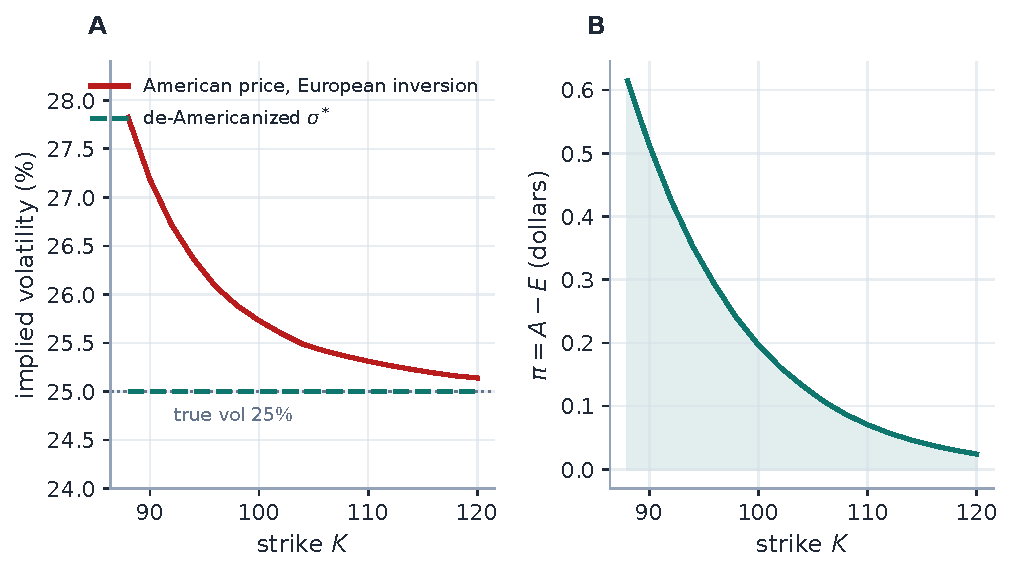
\includegraphics[width=\textwidth]{fig_deamst_bias.pdf}
\caption{The wrong-way demo on the running example (American calls, $6\%$
dividend yield, true vol $25\%$).  A: handing the American price to the
production European inversion books the premium as volatility --- up to
\deamstmaxbias\ vol bp, growing as the option goes in the money;
de-Americanization returns a flat $25\%$.  B: the premium itself in price
units --- \emph{cents}.  The damage is measured in vol basis points because
the wings divide by a small vega, not because the dollars are large.}
\label{fig:bias}
\end{figure}

\begin{figure}[H]
\centering
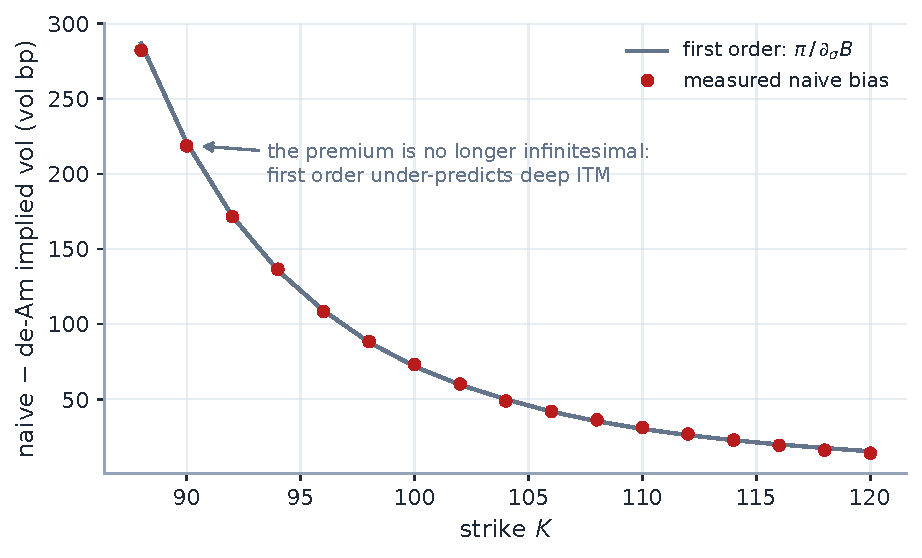
\includegraphics[width=0.82\textwidth]{fig_deamst_vega.pdf}
\caption{The dictionary, audited.  The measured naive bias (dots) against
the first-order prediction $\pi/\partial_\sigma\Black$ (line): agreement to
\deamstvegaotmerr\ vol bp out of the money, systematic under-prediction
deep in the money where $\pi$ is a finite, not infinitesimal, price move.
First-order vega reasoning locates the damage; only the full inversion
sizes it.}
\label{fig:vega}
\end{figure}

The machinery below engages only when a chain snapshot declares itself
American-exercise (set by the data layer; US-listed single-stock and ETF
chains in practice).  European snapshots --- index options, synthetic
chains --- skip every step byte-identically: invariant~1.

%======================================================================
\section{Where the premium lives: a little optimal stopping}
\label{sec:stopping}

Before removing $\pi$ it pays to know where it is --- because over much of
the strike--maturity plane it is \emph{exactly zero}, and the theory that
says so is short enough for a lecture to carry in full.  Write the
American value as an optimal-stopping problem over stopping times
$\vartheta\in\mathcal T_{[0,t]}$ of the price filtration,
\begin{equation}
A=\sup_{\vartheta\in\mathcal T_{[0,t]}}
\E\big[e^{-r\vartheta}\,g(S_\vartheta)\big],
\qquad g(s)=(s-K)^+\ \text{or}\ (K-s)^+,
\label{eq:stopping}
\end{equation}
under the risk-neutral measure \cite{PeskirShiryaev2006}.

\begin{proposition}[Dominance, both ways]
\label{prop:dominance}
$A\ge E$ and $A\ge g(S_0)$; hence $\pi=A-E\ge0$, and $A$ never trades
below intrinsic.
\end{proposition}

\begin{proof}
The stopping times $\vartheta\equiv t$ and $\vartheta\equiv0$ are both
admissible, and a supremum dominates every member of its feasible set.
\end{proof}

That one line already fixes two production conventions: the estimate of a
nonnegative premium may be clamped at zero (\cref{sec:pipeline}), and an
American quote \emph{below} intrinsic is not a premium puzzle but a broken
price (\cref{sec:cv} returns it as \texttt{nan}).  The substantive
question is when the inequality $A\ge E$ is an equality.

\begin{theorem}[Merton: no dividends, no premium]
\label{thm:merton}
For a call on an underlying paying no dividends, with $r\ge0$, early
exercise is never strictly optimal: $A=E$ and $\pi=0$
\cite{Merton1973}.
\end{theorem}

\begin{proof}
Let $E(s,u)$ denote the European call value with time $u$ left.  Convexity
of $x\mapsto(x-K)^+$ and Jensen's inequality under the martingale spot
(no dividends: $\E[e^{-ru}S_u\,|\,S_0=s]=s$) give
$E(s,u)\ge(s-Ke^{-ru})^+\ge s-K$, with strict inequality whenever $u>0$,
$K>0$ and $r>0$ (and weak throughout at $r=0$).  At any interior time the
American holder's continuation value is at least the European value of the
remaining claim, hence strictly above intrinsic: stopping early forfeits
value.  The supremum in \eqref{eq:stopping} is attained at
$\vartheta\equiv t$, which is the European contract.
\end{proof}

\begin{proposition}[Puts do carry a premium]
\label{prop:put}
For a put with $r>0$ there are states where $\pi>0$: whenever
$S<K(1-e^{-rt})$, exercise-now strictly beats any European continuation.
\end{proposition}

\begin{proof}
The European put is bounded by its discounted-strike cap, $E\le Ke^{-rt}$.
Deep enough in the money the intrinsic value exceeds that cap:
$K-S>Ke^{-rt}\iff S<K(1-e^{-rt})$.  Then
$A\ge K-S>Ke^{-rt}\ge E$.  Interest on the strike is earned by exercising
\emph{now}; waiting pays the option's remaining time value, which deep in
the money tends to zero while the interest does not.
\end{proof}

The same trade-off, run with dividends on the other side, makes the call
story symmetric: a dividend is value the call holder collects only by
exercising \emph{before} the ex-date, so cash dividends (or a carry yield
$q>r$) open a nonempty exercise region on deep in-the-money calls.  The
boundary between ``continue'' and ``exercise now'' is the \emph{free
boundary} of the obstacle problem --- an object with its own large
literature \cite{PeskirShiryaev2006} --- and \cref{fig:map} computes its
production shadow: the region of quotes whose entire value is intrinsic.

\begin{figure}[H]
\centering
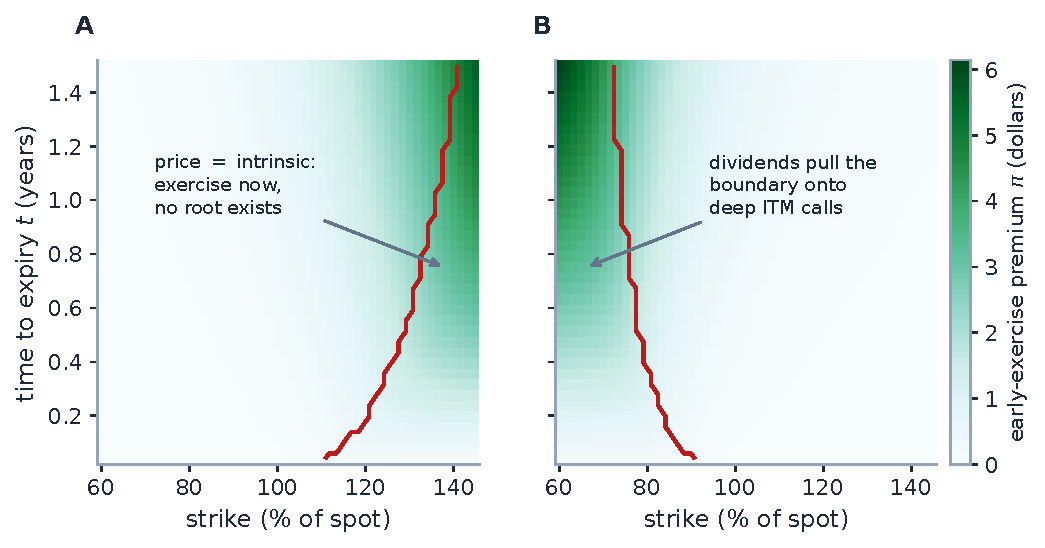
\includegraphics[width=\textwidth]{fig_deamst_map.pdf}
\caption{The premium mapped over the quote plane by the production tree
(true vol $25\%$).  A: puts at $r=4\%$, no dividends --- the premium
concentrates deep in the money and grows with maturity; right of the rust
boundary the price \emph{equals} intrinsic (at $t=0.5$, strikes beyond
$\deamstmapputbdry\%$ of spot; premium up to \$\deamstmapputeep).  In that
dead zone a quote carries no volatility information at all, and the
inversion of \cref{sec:cv} correctly refuses to invert it.  B: calls under
the running example's $6\%$ carry --- the mirror image: dividends pull the
exercise region onto deep ITM calls (below $\deamstmapcallbdry\%$ of spot
at $t=0.5$).  A call on a no-dividend name shows no shaded region at all
--- that is \cref{thm:merton} drawn.}
\label{fig:map}
\end{figure}

\paragraph{Exercise 1.}
Convince yourself the fitter needs no de-Americanization for calls on a
zero-dividend, zero-borrow name even though the chain is legally American:
show from \cref{thm:merton} that the root $\sigma^*$ of \cref{eq:deam}
then coincides with the naive European inversion up to tree error.  (This
is why \cref{fig:map}B needed dividends to be interesting --- and why the
premium machinery keys on the \emph{chain's} exercise style, not on any
per-quote guess about optimality.)

\begin{heuristic}
Why the fitter cares where $\pi$ lives: production fits the OTM side of
the book (\cref{sec:pipeline}), and \cref{thm:merton} plus
\cref{prop:put} say the OTM side is exactly where $\pi$ is small ---
OTM options have no intrinsic value to trade against carry.  The
\emph{large} premiums sit on ITM quotes production mostly discards.  The
honest size of the de-Americanization effect on the fitted population is
therefore \emph{a few} vol bp (\cref{sec:real}), not the hundreds the ITM
stress exhibits show --- and both numbers are worth knowing, because the
few-bp population is fitted against sub-vol-bp error budgets, and the
discarded population reappears whenever the forward solver or a user
selection touches an ITM quote.
\end{heuristic}

%======================================================================
\section{Where the subtraction sits}
\label{sec:pipeline}

De-Americanization is one stage of quote preparation.  For one (ticker,
expiry) the flow is: resolve $(\fwd,D)$ from the chain (put--call parity
plus the American de-bias of \cref{sec:carry}); keep the OTM side of the
book --- puts for $K<\fwd$, calls for $K\ge\fwd$, where the vega and the
tight relative spreads live --- and run the tick-noise and missing-side
screens; then, on American chains only, de-Americanize each surviving mid;
convert to normalized calls and total variance; optionally repair wing
convexity (\cref{sec:convex}); hand the result to the model layer.  The
implementation lives in \texttt{volfit/api/quotes.py}; everything below is
the mathematics of its three de-Am moves.

\subsection{One root per strike, spread preserved}

Given the American mid $P^{\mathrm m}$ at a strike, the pipeline solves for
the volatility $\sigma^*$ at which the tree of \cref{sec:tree} reprices it,
then reprices the \emph{European} leg at that same volatility:
\begin{equation}
A(\sigma^*)=P^{\mathrm m},\qquad
\hat\pi=\max\!\big(P^{\mathrm m}-E(\sigma^*),\,0\big),
\label{eq:eephat}
\end{equation}
and subtracts the \emph{same} $\hat\pi$ from bid, mid and ask.  Three
design decisions are packed into that line.  The clamp at zero is
\cref{prop:dominance} enforced against quote and tree noise --- the true
premium cannot be negative, so a negative estimate is noise; it is
one-sided by design, and \cref{sec:convex} prices what the asymmetry
costs.  One root per strike, rather than three, preserves the quoted
dollar spread exactly (invariant~2) at a third of the cost --- the
alternative, rooting bid and ask separately, would let tree error breathe
the spread.  And a quote the tree cannot invert keeps $\hat\pi=0$
(invariant~3): its raw band falls through to the European static-bound
filters, which will drop it if it is genuinely unusable.

\subsection{Into model space}

The shifted prices enter the ordinary European pipeline: normalization to
undiscounted forward units, put--call parity conversion of the OTM puts,
\begin{equation}
c=\frac{P}{D\fwd}\ \ \text{(calls)},\qquad
c=\frac{P}{D\fwd}+1-e^{\logm}\ \ \text{(puts)},
\label{eq:parity}
\end{equation}
then a strike-by-strike inversion to total variance $\tvar$.  Strikes whose
bid, mid or ask violates the static bounds $(1-e^{\logm})^+<c<1$ are
dropped (a one-sided band cannot be weighted), and a wing filter removes
strikes beyond $Z_{\max}=4$ ATM standard deviations.

\begin{remark}[The two clocks, once]
\label{rem:clocks}
Total variance is inverted from the \emph{price}, so it is
clock-independent; only the reported vol depends on the working clock,
$\mathrm{iv}=\sqrt{\tvar/\tau}$.  The $\sigma^*$ of \cref{eq:eephat} is a
calendar-time Black vol used \emph{transiently} inside the premium
estimate; the vol a user sees for the same quote can differ because
$\tau\ne t$ when event weighting is on (Note~00).  This is the first of
$\tau$'s two appearances; the second is the cache key of \cref{sec:cost},
and for the same reason.
\end{remark}

%======================================================================
\section{The pricing map}
\label{sec:tree}

\subsection{A tree for the obstacle problem}

The stopping problem \eqref{eq:stopping} needs a numerical method, and the
classical one is Cox--Ross--Rubinstein \cite{CoxRossRubinstein1979}:
approximate the diffusion by a binomial lattice and solve the stopping
problem by dynamic programming.  With $N$ steps of size $\Delta t=t/N$,
the spot moves by $u=e^{\sigma\sqrt{\Delta t}}$ or $d=1/u$, and matching
the risk-neutral drift fixes the up-probability
\begin{equation}
p=\frac{e^{(r-q)\Delta t}-d}{u-d},
\qquad 0<p<1
\iff \sigma\sqrt{\Delta t}>\abs{r-q}\,\Delta t .
\label{eq:crr_p}
\end{equation}
The condition on the right is the lattice's no-arbitrage requirement
$d<e^{(r-q)\Delta t}<u$: the one-step move must be able to out-run the
drift.  It fails only for extreme drift-to-vol ratios, and
\cref{sec:cv} shows how each code path treats the failure.  The value is
then the backward recursion
\begin{equation}
V^{(N)}_j=g(S_j),\qquad
V^{(m)}_j=\max\Big\{g(S_j),\;
e^{-r\Delta t}\big(p\,V^{(m+1)}_{j+1}+(1-p)\,V^{(m+1)}_{j}\big)\Big\},
\label{eq:rollback}
\end{equation}
--- projected dynamic programming: the discrete Bellman equation of
\eqref{eq:stopping}, with the $\max$ against the obstacle $g$ applied at
every node.  Drop the $\max$ and the same recursion prices the European
leg $E$.  Readers of Note~04 will recognize the family resemblance: the
rollback is a monotone scheme (each $V^{(m)}_j$ is a nonnegative
combination of the next layer, and $\max$ preserves order), which is the
discrete reason tree prices are stable, ordered, and free of invented
extrema.  Stripped of the dividend machinery the kernel is a dozen lines
(this listing reproduces the production \texttt{binomial\_price} at $q=0$
to $10^{-10}$; the European leg matches Black--Scholes to $2\times10^{-3}$
at this depth):

\begin{lstlisting}[caption={The CRR backward induction with early exercise
(distilled from \texttt{core/american.py}).},label={lst:crr}]
def crr_price(is_call, s, k, t, sigma, r, n=501, american=True):
    dt = t/n; u = np.exp(sigma*np.sqrt(dt)); d = 1/u
    p = (np.exp(r*dt) - d)/(u - d); disc = np.exp(-r*dt)   # risk-neutral up-prob
    sT = s * u**np.arange(-n, n+1, 2)                      # terminal spots
    v = np.maximum(sT-k, 0.0) if is_call else np.maximum(k-sT, 0.0)
    for m in range(n-1, -1, -1):                          # roll back one layer
        v = disc*(p*v[1:] + (1-p)*v[:-1])                 # continuation value
        if american:                                     # the obstacle:
            sM = s * u**np.arange(-m, m+1, 2)             #   max(continuation,
            v = np.maximum(v, sM-k if is_call else k-sM)  #       intrinsic)
    return v[0]
\end{lstlisting}

\subsection{Monotone in volatility, hence invertible}
\label{sec:monotone}

The inversion of \cref{sec:cv} treats $\sigma\mapsto A(\sigma)$ as a
scalar equation to be rooted.  For that to be well posed we need the map
to be increasing --- which is a theorem, with an honest scope.

\begin{proposition}[Monotonicity of the American price in volatility]
\label{prop:mono}
In the Black--Scholes model with convex vanilla payoff, the American value
is nondecreasing in $\sigma$ \cite{ElKarouiJS1998}: convexity of the
payoff propagates to the value function of the stopping problem, and a
comparison argument in the diffusion coefficient then orders the values.
Away from the intrinsic plateau the monotonicity is strict, so the root of
$A(\sigma)=P^{\mathrm m}$ is unique when it exists.
\end{proposition}

Two honest footnotes.  First, the proposition is about the continuous
problem; the discrete tree converges to it \cite{CoxRossRubinstein1979}
but a per-$N$ monotonicity proof is not carried here --- the
implementation's bracketed bisection requires only a sign change, which
the bracket-expansion loop of \cref{sec:cv} certifies before any halving.
Second, ``when it exists'': on the intrinsic plateau of \cref{fig:map}
--- a deep ITM quote priced \emph{at} its exercise floor --- no $\sigma$
reaches the quote from above, there is no root, and the honest answer is
``this quote contains no volatility'': the \texttt{NaN} lane.
\Cref{fig:root} draws all of this at once.

\begin{figure}[H]
\centering
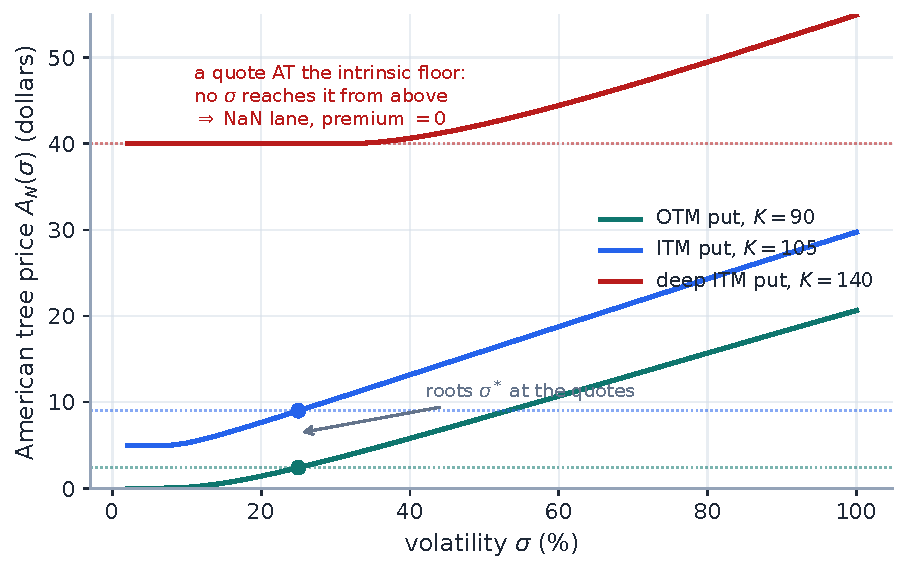
\includegraphics[width=0.82\textwidth]{fig_deamst_root.pdf}
\caption{The inversion, well posed and failing, on American puts
($r=4\%$, $t=0.5$, production tree).  For the OTM and moderately ITM
strikes $A(\sigma)$ is strictly increasing and crosses its quote (dots) at
a unique $\sigma^*$.  The deep ITM strike is pinned at intrinsic
(\$40) for every small $\sigma$: a market quote \emph{at} that floor is
below every model price on the bracket, no root exists, and the batch path
returns \texttt{NaN} --- premium zero, invariant~3 --- rather than
inventing a volatility.}
\label{fig:root}
\end{figure}

\subsection{The carry the tree runs on}
\label{sec:carry}

For a real single name a flat continuous yield is a crude proxy: the
call-side stopping decision of \cref{sec:stopping} keys on \emph{discrete
ex-dates}, not on a smear of carry.  Production therefore chooses, per
(ticker, expiry), one of two carry models for the tree
(\texttt{volfit/api/quotes.py}, \texttt{volfit/data/dividends.py}):

\begin{itemize}[leftmargin=1.6em]
\item \textbf{Discrete cash schedule, $q=0$.}  When the dividend model
supplies cash dividends $\delta_i$ with ex-dates $t_i\in(0,t]$, the tree
prices them by the escrowed-spot method \cite{Hull2018}.  Why escrow?  A
cash drop applied at the nodes breaks recombination: after an ex-date,
``up then down'' and ``down then up'' no longer meet, because the
subtracted cash is scaled differently by the subsequent multiplicative
moves, and the lattice explodes from $O(N)$ nodes per layer to $O(2^N)$
paths.  Escrowing instead diffuses the \emph{base}
$X_0=S-\sum_i\delta_ie^{-rt_i}$ --- a purely multiplicative, recombining
lattice --- and adds back the present value of the dividends \emph{not yet
paid} at each node before comparing against the obstacle, so exercise is
tested against the true cum-dividend spot.  The cash amounts are rescaled
by
\begin{equation}
\alpha=\frac{S-\fwd e^{-rt}}{\sum_i \delta_i e^{-rt_i}}
\label{eq:alpha}
\end{equation}
so that the escrowed-tree forward $(S-\mathrm{PV}_0)e^{rt}$ reproduces the
resolved forward \emph{exactly}: the timing stays the forecast, the
amounts bend to the market.  (On the running example of
\cref{fig:escrow}, a market forward $15$\,bp of carry under the forecast
rescales the cash by $\alpha=\deamstalpha$.)  A non-physical $\alpha$
($\le0$ or beyond a sanity cap) rejects the schedule.
\item \textbf{Continuous carry fallback.}  Otherwise the tree runs on the
$(r,q)$ implied by the resolved pair $(\fwd,D)$.
\end{itemize}
The two never coexist inside one tree, and \cref{eq:alpha} is what keeps
the cash choice consistent with a forward whose level partly reflects
yield-like far-tail effects.

\begin{remark}[The escrowed model is a displaced lognormal]
\label{rem:displaced}
The diffusing object under escrow is $S-\mathrm{PV}(\text{dividends})$,
so the model's spot distribution is a lognormal \emph{shifted} by the
escrow --- slightly skewed relative to the plain lognormal at the same
forward.  The premium estimate $\hat\pi$ inherits this modelling choice;
it is part of the ``exact in the model, approximate outside it'' honesty
of \cref{sec:cv}.
\end{remark}

\Cref{fig:escrow} shows why production pays for the discrete schedule
where it can get one: at the same forward, the cash tree and the yield
tree price materially different premia, and only the cash tree knows that
an option expiring \emph{before} the ex-date has no dividend to capture
--- \cref{thm:merton} switching on at a date, not fading in.

\begin{figure}[H]
\centering
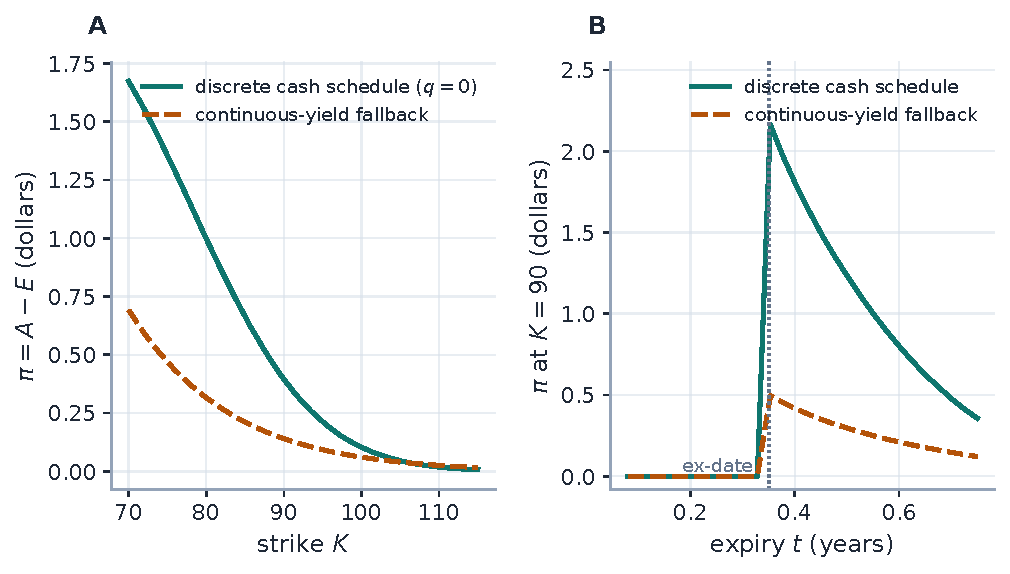
\includegraphics[width=\textwidth]{fig_deamst_escrow.pdf}
\caption{Same forward, different exercise value (production trees; one
\$3 dividend, ex-date at $0.35$y, $r=4\%$).  A: the call premium across
strikes under the forward-consistent cash schedule versus the
continuous-yield fallback --- the cash tree's premium is up to
$\deamstescrowratio\times$ larger, because a lump of value at a date is
worth more to an early exerciser than the same value smeared into carry.  B: the
premium at a fixed ITM strike as a function of expiry: under cash it is
\emph{zero} for every expiry before the ex-date (Merton's theorem applies
verbatim --- nothing to capture) and switches on at the date; the yield
model fades in smoothly and misses both regimes.  The kink is the
call-side ATM signature that motivates the joint refinement of
\cref{rem:circular}.}
\label{fig:escrow}
\end{figure}

\begin{remark}[The apparent circularity, resolved]
\label{rem:circular}
De-Americanization needs $(\fwd,D)$; but put--call parity --- the source
of $(\fwd,D)$ --- is an equality \emph{only for European options}, so raw
American mids bias the parity regression.  Production resolves the loop in
order: the parity regression runs first; then a \emph{coarse} de-Am pass
(\texttt{volfit/data/forwards.py}) de-biases it --- including, where the
de-Americanized put and call vols fail to join at the money, a rate
bisection that zeroes the gap (the joint $(r,\fwd)$ refinement; the
ATM-kink case file of Note~06); only then does the \emph{precise}
per-quote de-Americanization of this note run, under the refined carry.
The refinement needs the carry to a few bp, not the quote to sub-bp, so it
runs fewer bisections at coarser tolerance.
\end{remark}

%======================================================================
\section{The inversion as a control variate}
\label{sec:cv}

We can now say precisely how the unobservable is removed.  The move is a
one-dimensional root find,
\begin{equation}
\boxed{\;\text{find }\sigma^*:\ A(\sigma^*)=P^{\mathrm m},\quad
\text{return }\sigma^*\text{ as the European-equivalent Black vol,}\;}
\label{eq:deam}
\end{equation}
the standard desk workflow --- convert American quotes to pseudo-European
quotes, then calibrate a European model --- studied critically by
Burkovska et al.~\cite{Burkovska2018}: pragmatic and fast, exact in the
model, not exact outside it.

\begin{heuristic}
Why is the \emph{tree's} $\sigma^*$ the right European volatility?
Because the tree is a \emph{control variate} for the stopping feature.
The market price differs from the European price we want by a premium we
cannot observe; the tree supplies a model premium
$\pi_{\mathrm{tree}}(\sigma)=A(\sigma)-E(\sigma)$ as a function of
$\sigma$.  Subtracting it at the root,
\begin{equation}
P^{\mathrm m}
-\underbrace{\big[A(\sigma^*)-E(\sigma^*)\big]}_{\text{model premium at }\sigma^*}
= E(\sigma^*)\;\approx\;D\fwd\,\Black(\logm,{\sigma^*}^2t),
\label{eq:cv}
\end{equation}
where the equality uses the defining property
$A(\sigma^*)=P^{\mathrm m}$ and the final step is tree discretization
only.  Two cancellations happen at once: the market's premium cancels
against the model's, and the tree's \emph{level} error largely cancels
between its American and European legs --- the tree only has to price the
\emph{difference} well, and the difference is a smooth, slowly varying
functional of $\sigma$.  \Cref{sec:budget} measures exactly how much of
each cancellation survives discretization.
\end{heuristic}

\subsection{Failure semantics: loud scalar, silent batch}
\label{sec:failure}

A price below intrinsic (impossible for an American option,
\cref{prop:dominance}) or above the static cap ($S$ for a call, $K$ for a
put) yields \texttt{nan}, mirroring the fitter's convention for unusable
quotes.  The bracket's lower end is lifted just above the CRR drift floor
of \cref{eq:crr_p} --- production uses
$\max(10^{-4},\,1.5\,\abs{r-q}\sqrt{t/N})$ --- and the upper end doubles
until the model price clears the quote, capped at $\sigma=4$; a quote
never bracketed under the cap returns \texttt{nan}.

The scalar and batch paths then \emph{deliberately} differ.  The scalar
path (one quote, Brent's method, $N=\deamstscalarsteps$) \emph{raises} on
an invalid CRR probability: a single mispriced input should be loud.  The
batch path must survive mixed inputs, so invalid lanes --- static-bound
violations, the intrinsic-plateau puts of \cref{fig:root}, never-bracketed
quotes --- return \texttt{NaN} and the rest of the chain proceeds; quote
prep reads \texttt{NaN} as ``no premium estimate'', sets $\hat\pi=0$, and
leaves the untouched band to the European filters (invariant~3).

\paragraph{Exercise 2.}
Derive the drift floor: show from \cref{eq:crr_p} that $0<p<1$ is
equivalent to $\sigma>\abs{r-q}\sqrt{t/N}$, and evaluate it on the running
example's carry ($\abs{r-q}=4\%$, $t=0.5$, $N=\deamsteps$):
$\sigma_{\min}\approx0.2\%$, lifted $1.5\times$ by production.  Conclude
that the floor excludes only volatilities no equity quote reaches, yet
protects every tree the bisection prices.

%======================================================================
\section{The error budget, measured}
\label{sec:budget}

The returned $\sigma^*$ carries four error sources; a lecture should
separate them because they scale differently and are bought back by
different levers.

\begin{itemize}[leftmargin=1.6em,itemsep=1pt]
\item \textbf{Root tolerance.}  The batch path runs \deambisect\ halvings
of a bracket at most $4.0$ wide: $4\cdot2^{-\deambisect}\approx
2.4\times10^{-7}$ of $\sigma$, about $0.002$ vol bp --- negligible.
\item \textbf{Finite tree, two legs.}  Discretization enters twice, and
unequally.  The \emph{level} error of the American leg moves the root
itself; the \emph{European-leg} gap $E(\sigma^*)-D\fwd\Black$ survives in
the price handed downstream.  \Cref{fig:cancel} separates them on the
worked example: at the batch depth $N=\deamsteps$ the root carries
\deamstrootbp\ vol bp while the reported quote carries \deamstdepthbp\
(worst strike \deamstdepthmax); at the scalar depth
$N=\deamstscalarsteps$ the reported error drops to \deamstdepthbpscalar.
On the real chain this European-leg gap is directly visible as the small
\emph{negative} bias on selected OTM calls (median
$\deamstselcallmedian$\,bp, \cref{sec:real}) --- tree versus analytic
Black, not a negative premium.
\item \textbf{Carry and dividend model.}  A wrong forward, discount or
cash schedule biases $\sigma^*$ directly; de-Americanization inherits, and
cannot repair, its inputs (\cref{sec:carry}; the closing caution of
\cref{sec:real}).
\item \textbf{Market versus model.}  The CRR diffusion between ex-dates,
the displaced-lognormal escrow (\cref{rem:displaced}) and the one-sided
clamp of \cref{eq:eephat} are modelling choices; their measurable
footprint is the wing non-convexity that \cref{sec:convex} repairs.
\end{itemize}

\begin{figure}[H]
\centering
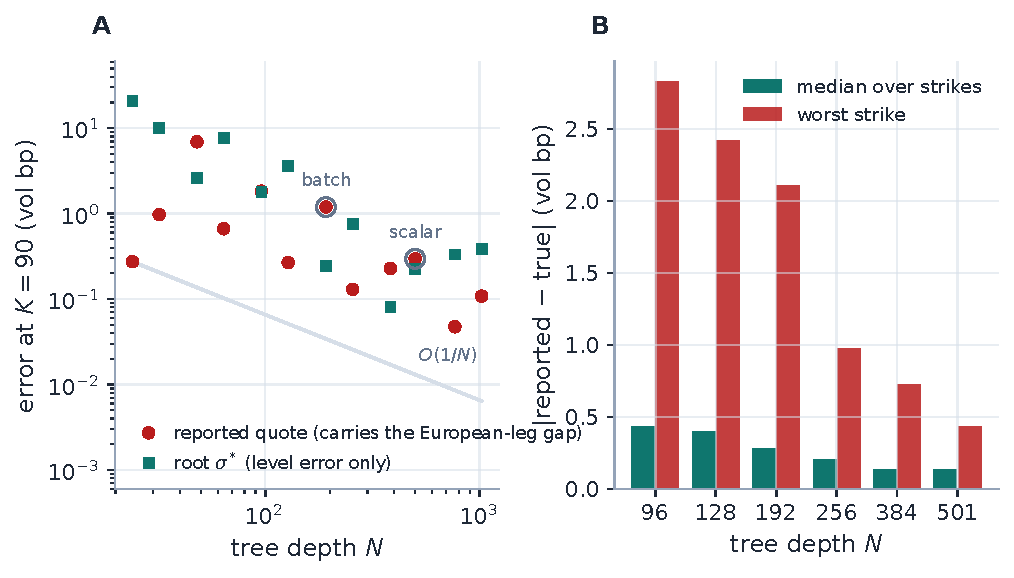
\includegraphics[width=\textwidth]{fig_deamst_cancel.pdf}
\caption{The cancellation, audited on the worked example (converged-tree
quote, production inversion at each depth).  A: at $K=90$, the root
$\sigma^*$ (teal) and the reported quote (rust) both converge like $1/N$
through the CRR even/odd sawtooth, but at any given depth the root is the
cleaner object --- the American-vs-European cancellation of \cref{eq:cv}
protects it, while the reported quote re-imports the European-leg gap.
B: the same end-to-end error aggregated across all strikes: the shipped
batch depth $\deamsteps$ holds the worst strike to \deamstdepthmax\ vol bp
and the median under $0.3$; halving the depth to $128$ roughly saves
half the work (the rollback is $O(N^2)$) but lifts the whole error
profile --- the depth is a numerical-target knob, not a speed dial.}
\label{fig:cancel}
\end{figure}

\begin{caution}
The batch depth was once nearly cut to $128$ as a cheap $2\times$ speed-up
--- the rollback is $O(N^2)$, so depth is the single most tempting dial in
the file.  Measured on the fitted population of the real chain
(\cref{sec:real}), the cut moves de-Americanized vols by a median
\deamstdepthrealmed\ and up to \deamstdepthrealmax\ vol bp --- material
against sub-vol-bp fitting budgets, and \emph{structured} (it loads on
low-vega strikes), so it changes answers, not just runtimes.  The depth is
held at $\deamsteps$ and the speed is bought where it does not touch the
numerical target: the kernel and the cache of \cref{sec:cost}.
\end{caution}

\paragraph{Exercise 3.}
From the budget above, explain why tuning the bisection count from $45$
to \deambisect\ sweeps was free ($<0.01$ vol bp, test-locked, a
$\sim1.8\times$ saving on the isolated de-Am rail) while the depth cut was
not: compare $4\cdot2^{-24}$ against the $N^{-1}$ tree terms at
$N=\deamsteps$, and note which term the extra $21$ halvings were polishing.

%======================================================================
\section{A worked example, by the numbers}
\label{sec:example}

Provenance in one line: every number in this note is regenerated by the
edition's figure generator at commit \texttt{\deamstgencommit}
(\deamstgendate), configuration archived alongside
(\nolinkurl{figures/deam_stopping_numbers.json}); the kernel timing is
read from the stored benchmark artifact of the original suite, never
re-timed.

\begin{example}[title={Case file: one strike of \cref{fig:bias}}]
Setup: American call, $S=100$, $K=\deamwexstrike$, $t=0.5$, $r=2\%$,
$q=6\%$, true volatility $\sigma=25\%$, scalar tree depth
$N=\deamstscalarsteps$.  The production tree prices
\[
A=\deamwexam,\qquad
E=\deamwexeu,\qquad
\pi=A-E=\deamwexeep .
\]
With a $6\%$ yield against a $2\%$ rate, exercising to capture the
dividend stream is genuinely valuable on an ITM call --- about $4.4\%$ of
this option's value sits in $\pi$.  Handing $A$ to the analytic European
inversion (production's normalization, $c=A/(D\fwd)$ at
$\logm=\log(K/\fwd)$) returns
\[
\sigma_{\text{naive}}=\deamwexnaive\%,
\]
a $+\deamwexbias$ vol bp phantom: the premium, booked as volatility.
Solving \cref{eq:deam} instead gives $\sigma^*=\deamwexdeam\%$ --- the
truth, to bisection tolerance.  Every number above is generated from
\texttt{core/american.py}; the full-strike sweep is \cref{fig:bias}.
\end{example}

%======================================================================
\section{The cost of a chain, and how it was made to vanish}
\label{sec:cost}

A lecture on a numerical method owes its audience the arithmetic.  One
rollback \eqref{eq:rollback} touches $N+(N-1)+\dots+1\approx N^2/2$ nodes:
one tree is $O(N^2)$.  One root is $\deambisect$ bisections plus a few
bracket expansions --- call it $30$ trees --- and one chain is a few
hundred roots: order $10^8$ multiply-adds at $N=\deamsteps$.  On modern
silicon that is tens of milliseconds of \emph{arithmetic}; the original
NumPy batch took a full second.  The gap was not the flops but the memory
system: vectorizing across quotes materializes $(n_{\text{quotes}}\times
m)$ slabs at every one of the $N$ steps, and the allocator, not the FPU,
was the bottleneck.  The compiled kernel inverts the loop order --- one
scalar tree per quote, no per-step allocation, precomputed power tables,
the escrow constants hoisted, a parallel loop over quotes --- and the same
public dispatch then runs \deamspeedup$\times$ faster.

\begin{perfbox}
On a \deamchainn-quote synthetic chain the kernel runs in \deamnumbams\,ms
versus \deamnumpyms\,ms for the NumPy fallback --- \deamspeedup$\times$.
The comparison is like-for-like: both timings call the public batch
dispatch (identical static screens, identical drift-floor bracket), the
NumPy leg by forcing the fallback; both paths run once untimed first (JIT
compile excluded) and the fastest of five repeats is reported; the
generator \emph{raises} unless the two paths return identical
finite/\texttt{NaN} lanes (\deamchainfinite\ of \deamchainn\ here --- the
rest are intrinsic-plateau puts, correctly \texttt{NaN} on both) and
identical roots (observed max $\abs{\Delta\sigma}=0$).  Measured on a
\deamthreads-thread desktop; this uniform synthetic chain parallelizes
especially well --- the documented figure on wide \emph{real} chains is
$\sim60\times$.  Without Numba the fallback serves with identical
results.
\end{perfbox}

The second lever is not faster code but \emph{less} code run.  The
de-Americanized, inverted quotes depend only on the \emph{data} entering
quote preparation --- never on any fit setting --- so the pipeline
memoizes each node's prepared quotes on a content-digest key built from
(ticker, expiry, raw-chain version, forward, discount, cash-dividend
digest, $t$, $\tau$, as-of).  Each entry is there for a reason a reader
can now predict: the forward and discount absorb forward policy and
manual edits; the cash digest absorbs the dividend model and rate;
calendar $t$ drives the tree; and $\tau$ appears for the reason of
\cref{rem:clocks} --- the cached band \emph{reports} vols on the event
clock, so an event edit must re-key.  A change to any of these re-runs
the trees; model choice, penalties, weights and optimizer tuning do not
(invariant~5).  The de-Am cost is thus paid once per genuine data change
and is \emph{free across an entire calibration sweep} --- a
complexity-class change, worth more than any constant factor the kernel
can buy.  A conservative pre-screen (non-positive bids, a buffered wing
cut) additionally drops quotes that cannot survive the static bounds
before any tree prices them, and is output-preserving by construction.

%======================================================================
\section{The wings: an approximate projection}
\label{sec:convex}

De-Americanization inverts each strike \emph{independently} --- its own
root \eqref{eq:deam}, its own clamp \eqref{eq:eephat} --- with no coupling
across strikes.  That independence is what makes the kernel embarrassingly
parallel; its price is that nothing enforces cross-strike coherence on the
output.  Writing the undiscounted call as $C(K)=\E[(S_t-K)^+]$, its second
derivative in strike is the risk-neutral density,
$\partial_{KK}C=f_{S_t}(K)\ge0$: \emph{convexity of the call curve in
strike is exactly the no-butterfly condition}.  On a discrete grid the
test is the divided second difference
\begin{equation}
\Delta^2_i=\frac{C_{i-1}(K_{i+1}-K_i)-C_i(K_{i+1}-K_{i-1})+C_{i+1}(K_i-K_{i-1})}
{K_{i+1}-K_{i-1}}\;\ge\;0 .
\label{eq:bfly}
\end{equation}
To be precise about the mechanism: per-strike inversion does not by itself
create arbitrage --- if the inputs were exactly consistent with one
arbitrage-free model, the outputs would be too.  The non-convexity is
\emph{injected}: by quote noise in sparse wings, by the one-sided
$\max(\hat\pi,0)$ clamp (a strike-local, asymmetric perturbation), by
finite-tree error, and by carry mismatch --- and per-strike inversion
simply has no cross-strike coupling with which to absorb any of it.  The
violations concentrate in the sparse, low-vega wings, handing every
downstream model a genuine (small) butterfly arbitrage as \emph{input} ---
the seed of the put-wing violation Note~03 dissects.

\begin{example}[title={Case file: the repair that moved the money}]
\textbf{Setup.}  The first repair projected the \emph{whole} call curve
onto the convex cone with a free global affine part --- the
mathematically obvious $\ell^2$ projection.

\textbf{Failure.}  A visible ATM smile gap opened on live SPY and NVDA.

\textbf{Diagnosis.}  Repairing a wing dip with a free global affine part
re-tilts the baseline: the projection moved the at-the-money prices it had
no business touching.  The moves were sub-penny --- \emph{small} in vol at
the money, where vega peaks --- but the ATM core is where quotes are
densest, spreads tightest and fit weight heaviest, and the coherent shift
opened a discontinuity against neighbouring untouched quotes.

\textbf{Fix.}  Reverted; redesigned wing-only (below), with the core held
byte-identical \emph{by construction} --- invariant~4 exists because of
this incident.

\textbf{Verdict.}  The lesson is about locality, not vega: \emph{a repair
aimed at a region the data cannot pin down must be structurally incapable
of moving the region it can.}  Note~04's convex-wing case file and
Note~09's tapered enforcement are the same principle wearing other
clothes.
\end{example}

The shipped repair (\texttt{volfit/calib/convex\_deam.py}) is therefore
\emph{wing-only, band-constrained} and --- honestly --- \emph{approximate}.
It acts on the normalized OTM call curve after the parity conversion
\eqref{eq:parity}.  Strikes in the core $\abs{z}\le Z_{\mathrm{core}}=1$
are held byte-identical.  Each wing, anchored at its core boundary, is
replaced by an approximation to the $\ell^2$-closest curve that is
simultaneously convex and inside the quoted band --- the projection onto
the intersection of two convex sets,
\begin{equation}
\mathcal C=\{\hat C\ \text{convex, leaving the anchor no flatter than the
core}\},\qquad
\mathcal B=\{C^{\mathrm b}\le\hat C\le C^{\mathrm a}\},
\label{eq:sets}
\end{equation}
computed by \emph{at most 25 iterations} of Dykstra's alternating
projection \cite{BoyleDykstra1986} --- the cone step a
nonnegative-hinge least squares, the band step a clip.  Dykstra rather
than plain alternation because plain von~Neumann alternation between
convex sets converges to \emph{a} point of the intersection, not to the
\emph{closest} one; Dykstra's correction terms restore the projection.
The honesty ledger, stated once and plainly: the implementation does not
certify $\mathcal C\cap\mathcal B\ne\emptyset$ (a wing whose
convexification demands leaving the band has no exact solution; the
iterate then lands near the band); it does not post-check global convexity
of the assembled curve; and it cannot, by construction, repair a violation
\emph{inside} the held-fixed core.  A common per-strike shift is applied
to bid, mid and ask --- the spread survives, invariant~2 again --- and the
repaired band is re-inverted to total variance.

\begin{heuristic}
Why the band constraint is load-bearing.  Plain convex projection of an
illiquid, genuinely non-convex wing is free to push a price all the way to
the static no-arbitrage boundary --- and a wing call price at that
boundary inverts to an absurd volatility (a put wing was once watched
jumping from $27\%$ to $104\%$, itself violating Lee's moment bound;
Note~03), detonating the downstream fit.  Confining the repair to the
quoted spread bounds the correction by the market's own stated
uncertainty: a price may move exactly as far as the quote is genuinely
ambiguous, and no further.
\end{heuristic}

The repair is gated American-only and short-circuits on any curve already
convex to a tolerance of $10^{-3}$ in normalized price (\cref{app:atlas}).
The threshold is calibrated to an observed gap in the data: dense liquid
chains carry only $\sim10^{-4}$ de-Am rounding curvature (the captured
delayed-tier SPY fixture of \cref{sec:real} quotes tick-wide spreads,
median
\ensuremath{\deamstliqmant\times10^{\deamstliqexp}} normalized --- an
order below the gate), while
genuinely arbitraged illiquid wings run $10^{-3}$ to $10^{-2}$.  Liquid
names are therefore \emph{never} touched (byte-identical), and only real
wing arbitrage is repaired --- roughly one American node in eight, in the
production ablations.  On those nodes the ablation found the repair both
reduces the fitted arbitrage and \emph{lowers} the in-sample error --- the
model no longer chases the arbitraged quotes --- and it composes with
Note~03's output-side $g\ge0$ penalty rather than duplicating it: the
repair removes the arbitrage at the \emph{source}, and running both
attains the penalty's arbitrage removal at a fraction of its standalone
in-sample cost.

\begin{figure}[H]
\centering
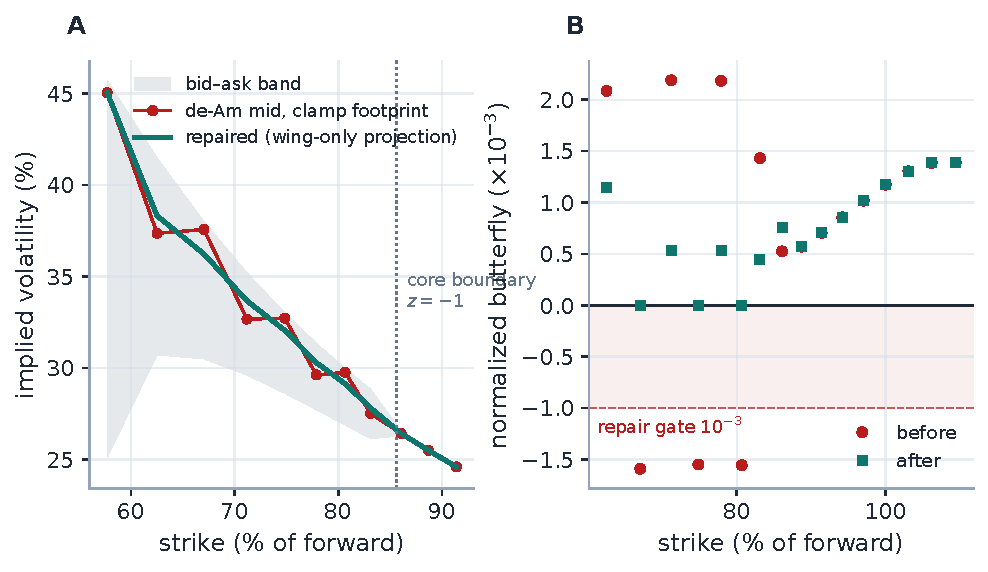
\includegraphics[width=\textwidth]{fig_deamst_convex.pdf}
\caption{The mechanism, staged where it actually operates (production
repair on a constructed illiquid wing --- the real fixture's tick-wide
bands cannot host a genuine violation, which is itself the liquid-gate
story).  A: a sparse put wing whose mids carry a one-sided clamp-scale
footprint inside a realistic bid--ask band; the projection returns a
convex wing \emph{inside the band}, anchored at the $z=-1$ boundary, and
the core to the right moves by exactly \deamstcvxcore.  B: the divided
second differences \eqref{eq:bfly}: before, dipping to
$\deamstcvxbefore\times10^{-3}$ --- through the $10^{-3}$ gate; after,
convex to machine precision
(\ensuremath{\deamstcvxaftermant\times10^{\deamstcvxafterexp}}).  The
largest vol move used to buy that convexity is \deamstcvxmove\ vol bp,
paid entirely inside the wing's quoted spread.}
\label{fig:convex}
\end{figure}

%======================================================================
\section{Real chains, honestly labelled}
\label{sec:real}

The synthetic example controls the truth; \cref{fig:real,fig:realsel}
show the effect on live market prices, nothing simulated --- and on two
deliberately different populations, because the single most misquotable
number in this subject is ``the de-Americanization effect'' with the
population left unsaid.

\paragraph{The stress exhibit (\cref{fig:real}).}
Every two-sided put of one captured SPY expiry (the Massive true-weekly
fixture, as-of 2026-06-25; the December-2026 expiry, strikes
$55$--$138\%$ of spot) is inverted both ways: naively through the analytic
European Black formula, and through the American tree \eqref{eq:deam}.
Since $\pi$ has price units, the wedge between the curves is the
\emph{model-implied} vol effect of the premium.  Out of the money the two
agree to a few vol bp; in the money the wedge runs to a median
\deamstrealmedianitm\ vol bp across the \deamstrealnitm\ ITM puts, up to
\deamstrealmaxbias.  But this population is \emph{not what the fitter
fits}: production keeps the OTM side only, so the ITM puts carrying the
headline wedge are --- in all but the thin band between spot and forward
--- exactly the quotes production \emph{discards} in favour of their OTM
call twins.  \Cref{fig:real} is an economic stress illustration of what
skipping de-Americanization would do to the discarded side, not a
statement of fit exposure.  \Cref{prop:put} told us in advance this is
where the premium had to be.

\begin{figure}[H]
\centering
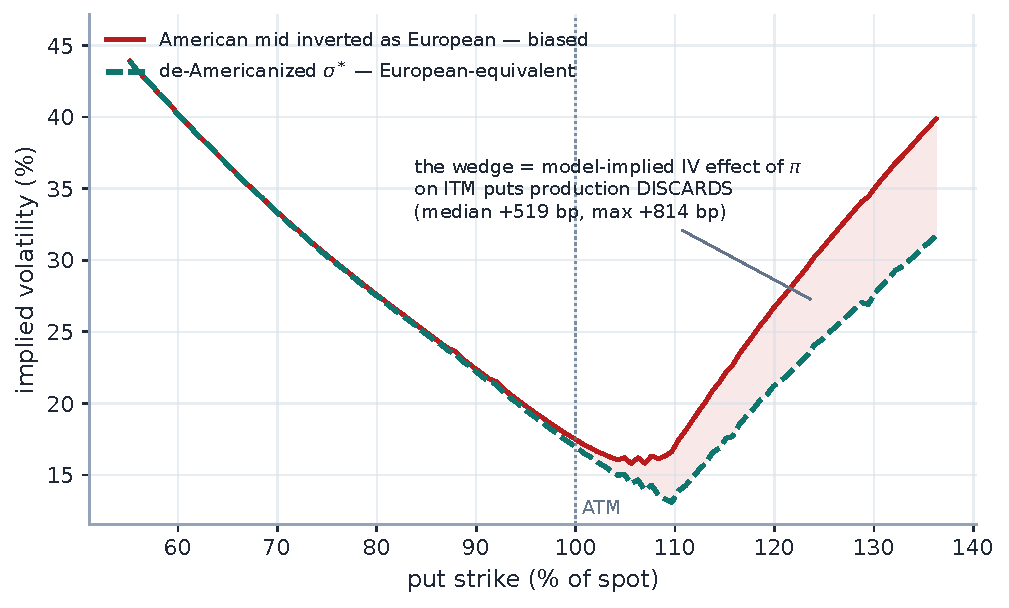
\includegraphics[width=0.82\textwidth]{fig_deamst_real.pdf}
\caption{Real market data, one live SPY expiry (Massive capture, as-of
2026-06-25, December-2026): every two-sided put mid inverted as if
European versus de-Americanized.  The ITM wedge --- median
\deamstrealmedianitm\ vol bp, up to \deamstrealmaxbias\ --- is the
model-implied vol effect of the premium on a side production almost
entirely \emph{discards}: a stress exhibit, not the fitted population
(that is \cref{fig:realsel}).  Carry supplied ($r=4.3\%$, $q=1.2\%$)
because the delayed capture's parity carry is unusable (Note~06).}
\label{fig:real}
\end{figure}

\paragraph{The fitted population (\cref{fig:realsel}).}
The same two-way inversion on the quotes production actually selects ---
\deamstseln\ OTM puts and calls of the same expiry, after the tick floor
and the $Z_{\max}$ wing filter --- moves the implied vol by a median
$\abs{\cdot}$ of \deamstselabsmedian\ vol bp, maximum \deamstselmax\
(selected OTM puts: median $\deamstselputmedian$\,bp, max
$\deamstselputmax$; selected OTM calls: median
$\deamstselcallmedian$\,bp, max $\deamstselcallmax$).  This is the honest
statement of what de-Americanization is worth on a liquid, moderate-carry
ETF chain at six months: a few vol bp in the body, tens in the put wing
--- material against sub-vol-bp error budgets, an order of magnitude
below the stress exhibit.  The small \emph{negative} call-side values are
the finite-tree line of \cref{sec:budget}'s budget, not a negative
premium.  Single names with hard dividends and higher rates sit between
the two panels.

\begin{figure}[H]
\centering
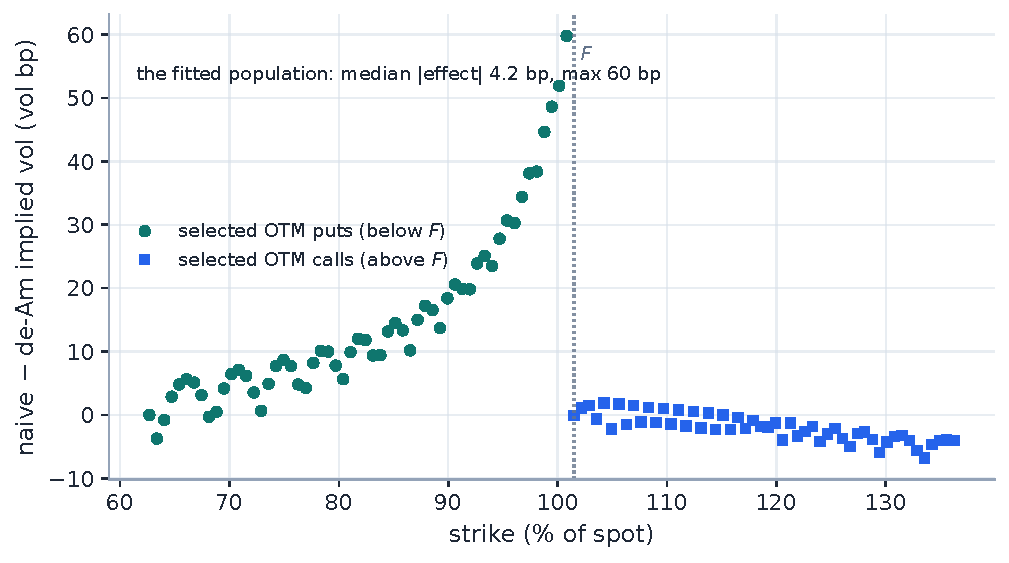
\includegraphics[width=0.82\textwidth]{fig_deamst_realsel.pdf}
\caption{The same expiry, restricted to the quotes production actually
fits (OTM puts below $\fwd$, OTM calls above): a median $\abs{\cdot}$ of
\deamstselabsmedian\ vol bp, max \deamstselmax\ in the put wing --- the
fit's real de-Am exposure, an order of magnitude below the discarded-ITM
stress exhibit.  The gentle put-side rise toward the money and the flat,
slightly negative call side are both predicted by
\cref{sec:stopping,sec:budget}: premium from \cref{prop:put}, tree error
from the European leg.}
\label{fig:realsel}
\end{figure}

One honesty note on inputs: the delayed-tier capture's parity-implied
carry is unphysical (Note~06 documents how such feeds synthesize chains
from per-contract vols at $\fwd=S$, $D=1$, destroying parity
information), so the carry here is supplied explicitly --- $r=4.3\%$
money-market, $q=1.2\%$ SPY dividend yield (mid-2026) --- a live instance
of the caution below.

\begin{caution}
What the model does and does not cover.  The tree supports a
deterministic scheduled cash-dividend path (escrowed, forward-consistent
via \cref{eq:alpha}) \emph{or} an equivalent continuous-carry fallback,
with a CRR diffusion between ex-dates.  It does not model dividend jumps,
uncertain dividend timing or amounts, stochastic rates, or stochastic
borrow.  And $\sigma^*$ is only as good as the resolved forward and
dividend inputs (Note~06): the method removes the \emph{early-exercise}
bias; it cannot repair a wrong forward.
\end{caution}

%======================================================================
\section{What is genuinely original here}
\label{sec:original}

The optimal-stopping theory is classical
\cite{Merton1973,PeskirShiryaev2006}, the control-variate reading of tree
inversion is folklore, and the critical literature is Burkovska et
al.~\cite{Burkovska2018}.  The contributions of this implementation are
discipline and measurement:
\begin{enumerate}[leftmargin=1.6em]
\item the \emph{allocation-free compiled kernel} behind an unchanged
public dispatch, with the agreement gate (identical \texttt{NaN} lanes,
identical roots) asserted before any speed number is reported;
\item the \emph{prepared-quote content cache}, which scopes de-Am cost to
genuine data changes rather than fit iterations --- a complexity-class
change, not a constant factor;
\item the \emph{measured} depth-and-bisection tuning: bisections cut
$45\to\deambisect$ at $<0.01$ vol bp, the depth cut to $128$ \emph{refused}
at a measured median \deamstdepthrealmed/max \deamstdepthrealmax\ vol bp
on the real fitted population;
\item the \emph{wing-only, band-constrained convex repair} with the
core held byte-identical by construction --- the redesign the reverted
global projection forced.
\end{enumerate}
The natural next step --- documented, not shipped --- is seeding the
bracket with an analytic American approximation (Barone-Adesi--Whaley
\cite{BaroneAdesiWhaley1987} or Bjerksund--Stensland
\cite{BjerksundStensland2002}) so each tree starts near its root: seeds,
not answers, so no contract changes.

%======================================================================
\section{Limitations}
\label{sec:limits}

Where the guarantees stop, gathered in one place.  De-Americanization is
exact \emph{in the model} and only there \cite{Burkovska2018}: the CRR
diffusion, the deterministic escrowed dividends
(\cref{rem:displaced}), and the flat per-expiry carry are all modelling
choices inside $\hat\pi$.  \Cref{prop:mono}'s monotonicity is a
continuous-problem theorem; the tree inherits it only through convergence,
and the implementation leans on bracketing, not monotonicity.  The clamp
in \cref{eq:eephat} is deliberately one-sided; its footprint is the wing
non-convexity of \cref{sec:convex}, and the repair that removes it is
approximate (capped Dykstra, no intersection certificate, core violations
out of scope by design).  The premium estimate inherits the resolved
forward and dividend inputs and cannot repair them.  And the intrinsic
plateau is a hard information boundary: a quote at its exercise floor
contains no volatility, and no method --- this one included --- can
extract what is not there.

\appendix
%======================================================================
\section{Hyperparameter atlas}
\label{app:atlas}

\begin{longtable}{p{0.26\textwidth}p{0.14\textwidth}p{0.52\textwidth}}
\caption{De-Americanization hyperparameters (all hidden / internal).}\label{tab:atlas}\\
\toprule Constant & Default & Role\\ \midrule
\endfirsthead \toprule Constant & Default & Role\\ \midrule \endhead
\texttt{DEFAULT\_STEPS} & $\deamstscalarsteps$ & Scalar CRR depth; European
leg matches Black to $\sim10^{-5}$.\\
\texttt{DEFAULT\_BATCH\_STEPS} & $\deamsteps$ & Batch/kernel tree depth
(\cref{sec:budget}'s caution).\\
\texttt{BATCH\_BISECTIONS} & $\deambisect$ & Bracketed-bisection sweeps
($\sim0.002$ vol bp).\\
\texttt{SIGMA\_LO} & $10^{-4}$ & Lower vol bracket floor; production lifts
it above the CRR drift floor,
$\max(10^{-4},\,1.5\,\abs{r-q}\sqrt{t/N})$.\\
\texttt{SIGMA\_HI} & $4.0$ & Upper vol bracket cap (bracket doubles up to
it).\\
escrow PV & --- & Discrete-cash escrowed-spot lattice, forward-consistent
rescale \cref{eq:alpha}, cap $\alpha\le5$.\\
pre-screen buffer & $1.5\times$ & Wing buffer for the conservative
bid/bounds pre-screen (output-preserving).\\
prepared-quote key & --- & Cache key: (ticker, expiry, raw-chain
version, forward, discount, dividend digest, $t$, $\tau$, as-of).\\
\texttt{convex\_deam} & \texttt{true} & Enable the wing-only convex
repair (\cref{sec:convex}); American chains only, European a no-op.\\
$Z_{\text{core}}$ & $1.0$ & ATM core half-width (units of
$\sqrt{\tvar_{\atm}}$) held byte-identical by the repair.\\
\texttt{CONVEX\_TOL} & $10^{-3}$ & Convexity short-circuit: a curve convex
to this (normalized price) is left untouched.\\
Dykstra iterations & $25$ & Cap on the alternating projection
(approximate, not certified).\\
$Z_{\max}$ & $4.0$ & Post-inversion wing filter (ATM standard
deviations).\\
\bottomrule
\end{longtable}

%======================================================================
\section{Performance notes}
\label{app:perf}

Machine-dependent numbers live here, with their protocol.

\begin{enumerate}[leftmargin=1.6em]
\item \textbf{Numba kernel} (\cref{sec:cost}).  Single scalar CRR per
quote, no per-step allocation, precomputed powers, parallel loop over
quotes; measured \deamspeedup$\times$ over the NumPy fallback on a
\deamchainn-quote synthetic chain (\cref{tab:time}; $\sim60\times$
documented on wide real chains).  Both paths through the public dispatch;
identical roots asserted before the number is reported; graceful NumPy
fallback when Numba is absent.
\item \textbf{Bisection tuning.}  $45\to\deambisect$ sweeps, $<0.01$ vol
bp drift (test-locked), $\sim1.8\times$ on the isolated de-Am rail.
\item \textbf{Depth: measured and refused.}  Batch depth $128$ evaluated
as a $\sim2\times$ lever and rejected at a measured median
\deamstdepthrealmed/max \deamstdepthrealmax\ vol bp shift on the real
fitted population (\cref{sec:budget}).
\item \textbf{Prepared-quote content cache.}  De-Am re-runs only on a
genuine data change, never on fit-setting changes --- free across a
calibration sweep.
\item \textbf{Output-preserving pre-screen.}  Drops unusable quotes before
any tree prices them; by construction changes no surviving result.
\item \textbf{Future (not shipped).}  BAW / Bjerksund--Stensland analytic
bracket seeds to start each tree near its root.
\end{enumerate}

\begin{table}[H]
\centering
\caption{De-Americanizing a \deamchainn-quote synthetic chain
(\deamchainfinite\ invertible on both paths, identical roots;
$\deamsteps$-step trees, \deambisect\ bisections; one untimed warm-up per
path, fastest of five repeats, \deamthreads\ threads).  Timing read from
the stored benchmark artifact; never re-timed by this edition.}
\label{tab:time}
\begin{tabular}{lrr}
\toprule
Path & time (ms) & relative\\
\midrule
NumPy fallback (same dispatch) & \deamnumpyms & $1\times$\\
Numba kernel & \deamnumbams & \deamspeedup$\times$\\
\bottomrule
\end{tabular}
\end{table}

%======================================================================
\section{Traceability}
\label{app:trace}

\begingroup
\small
\setlength{\tabcolsep}{4pt}
\renewcommand{\arraystretch}{1.15}
\begin{longtable}{@{}p{0.40\textwidth}p{0.12\textwidth}p{0.44\textwidth}@{}}
\caption{Claim $\to$ equation $\to$ code $\to$ test.}\label{tab:trace}\\
\toprule Claim & Equation & Code anchor \newline \emph{Test anchor}\\ \midrule
\endfirsthead
\toprule Claim & Equation & Code anchor \newline \emph{Test anchor}\\ \midrule
\endhead
$\sigma^*$ root = de-Americanized Black vol; static-bound / drift-floor
\texttt{NaN} semantics & \eqref{eq:deam}, \eqref{eq:cv} &
\nolinkurl{volfit/core/american.py}\newline
\nolinkurl{tests/test_american.py}\\
\addlinespace
Spread-preserving $\hat\pi$ shift of bid/mid/ask; OTM selection; parity
conversion & \eqref{eq:eephat}, \eqref{eq:parity} &
\nolinkurl{volfit/api/quotes.py}\newline
\nolinkurl{tests/test_quotes_deam.py}\\
\addlinespace
$\deambisect$-bisection drift $<0.01$ vol bp vs the 45-sweep baseline &
--- & \nolinkurl{volfit/core/american.py}\newline
\nolinkurl{tests/test_quotes_deam.py}\\
\addlinespace
Escrowed cash schedule, forward-consistent rescale & \eqref{eq:alpha} &
\nolinkurl{volfit/data/dividends.py}\newline
\nolinkurl{tests/test_discrete_deam.py}\\
\addlinespace
Kernel $=$ NumPy fallback to tree rounding (incl.\ cash dividends) & ---
& \nolinkurl{volfit/core/american_numba.py}\newline
\nolinkurl{tests/test_american_numba.py}\\
\addlinespace
Prepared-quote cache: invalidation table & --- &
\nolinkurl{volfit/api/service.py}\newline
\nolinkurl{tests/test_prepared_cache_key.py}\\
\addlinespace
Wing repair: ATM core byte-identical, band-stay, convexity gate &
\eqref{eq:bfly}, \eqref{eq:sets} &
\nolinkurl{volfit/calib/convex_deam.py}\newline
\nolinkurl{tests/test_convex_deam.py}\\
\addlinespace
Joint $(r,\fwd)$ American de-bias joins the ATM sides & --- &
\nolinkurl{volfit/data/forwards.py}\newline
\nolinkurl{tests/test_forward_debias.py}\\
\bottomrule
\end{longtable}
\endgroup

%======================================================================
\section{Reference implementation: convexity building blocks}
\label{app:ref}

The convexity test \eqref{eq:bfly} and the convex-cone half of the wing
repair are compact; the listing shows these two \emph{building blocks},
not the shipped repair.  \texttt{min\_butterfly} is the divided second
difference (minimum $\ge0$ iff the curve is butterfly-free);
\texttt{convex\_fit} is the cone projection --- the $\ell^2$-closest
convex curve leaving the core anchor, written as an affine part plus
nonnegative hinge knots, so $\delta_j\ge0$ \emph{is} the convexity
constraint.  The production module composes \texttt{convex\_fit} with the
bid/ask clip inside the capped Dykstra alternation of \cref{sec:convex}
and additionally handles duplicate strikes and the core/wing gating ---
none of which is shown.  Both listings were executed against their
production counterparts on the demo wing of \cref{fig:convex} before this
note was committed: agreement to $10^{\deamstrefagree}$ (floating-point
identity), asserted by the edition's generator on every run.

\begin{lstlisting}[caption={The no-butterfly test and the convex wing fit
(distilled from \texttt{calib/convex\_deam.py}).}]
def min_butterfly(K, C):                     # >= 0  <=>  C convex in strike (no bfly)
    a, b = K[1:-1]-K[:-2], K[2:]-K[1:-1]     # left / right strike gaps
    fly = C[:-2]*b - C[1:-1]*(a+b) + C[2:]*a # divided second difference
    return (fly / (a+b)).min()

def convex_fit(u, c, slope_floor):           # L2-closest convex curve, anchor c[0]
    cols = [u] + [np.maximum(u-u[j], 0.0) for j in range(1, len(u)-1)]
    A = np.column_stack(cols)                # [u, (u-u_j)_+ ...] : affine + hinges
    lb = np.zeros(A.shape[1]); lb[0] = slope_floor   # leaving slope >= core; delta_j >= 0
    x = lsq_linear(A, c - c[0], bounds=(lb, np.inf)).x
    return c[0] + A @ x                       # convex by construction (delta_j >= 0)
\end{lstlisting}

\begin{thebibliography}{9}
\bibitem{CoxRossRubinstein1979} J.~Cox, S.~Ross and M.~Rubinstein.  Option
pricing: a simplified approach.  \emph{J.\ Financial Economics},
7(3):229--263, 1979.
\bibitem{Merton1973} R.~Merton.  Theory of rational option pricing.
\emph{Bell J.\ Economics and Management Science}, 4(1):141--183, 1973.
\bibitem{PeskirShiryaev2006} G.~Peskir and A.~Shiryaev.  \emph{Optimal
Stopping and Free-Boundary Problems}.  Birkh\"auser, 2006.
\bibitem{ElKarouiJS1998} N.~El~Karoui, M.~Jeanblanc-Picqu\'e and
S.~Shreve.  Robustness of the Black and Scholes formula.
\emph{Mathematical Finance}, 8(2):93--126, 1998.
\bibitem{Hull2018} J.~Hull.  \emph{Options, Futures, and Other
Derivatives}.  Pearson, 10th edition, 2018.  (Escrowed-dividend binomial
trees.)
\bibitem{BoyleDykstra1986} J.~Boyle and R.~Dykstra.  A method for finding
projections onto the intersection of convex sets in Hilbert spaces.
\emph{Advances in Order Restricted Statistical Inference}, Springer,
1986.
\bibitem{BaroneAdesiWhaley1987} G.~Barone-Adesi and R.~Whaley.  Efficient
analytic approximation of American option values.  \emph{J.\ Finance},
42(2):301--320, 1987.
\bibitem{BjerksundStensland2002} P.~Bjerksund and G.~Stensland.  Closed
form valuation of American options.  Working paper, NHH, 2002.
\bibitem{Burkovska2018} O.~Burkovska et al.  Calibration to American
options: numerical investigation of the de-Americanization method.
\emph{arXiv:1611.06181}.
\end{thebibliography}

\end{document}
